% ----------------------------------------------------------------------------------------------------------------------------------
% Advanced pgBackRest
% ----------------------------------------------------------------------------------------------------------------------------------
\def\mytitle{Advanced pgBackRest}
\def\mysubject{}
\def\myevent{PGConf NYC 2023}
\def\myauthor{David Steele}
\def\myemail{}
\def\mydate{October 4, 2023}

% Suppres navigation bars
\def\mysuppressnav{}

% Include Crunchy template
\def\mytemplatepath{/template/}
\input{\mytemplatepath crunchy-template.tex}

% Agenda
\begin{frame}[fragile]
    \frametitle{Agenda}
    \tableofcontents
\end{frame}

% ----------------------------------------------------------------------------------------------------------------------------------
\section{Introduction}

\begin{frame}[fragile]
    \frametitle{About the Speaker}

    \begin{itemize}
        \item Principal Architect at Crunchy Data, the Trusted Open Source Enterprise PostgreSQL Leader.
        \item Actively developing with PostgreSQL since 1999.
        \item Maintainer of pgBackRest and pgAudit.
        \item PostgreSQL Contributor.
    \end{itemize}
\end{frame}

% ----------------------------------------------------------------------------------------------------------------------------------
\section{What is pgBackRest?}

\begin{frame}[fragile]
    \frametitle{What is pgBackRest?}

    pgBackRest aims to be a reliable, easy-to-use backup and restore solution that can seamlessly scale up to the largest databases and workloads by utilizing algorithms that are optimized for database-specific requirements.
    \\\vspace{1em}
    Major features:

    \begin{itemize}
        \item Parallelism and asynchronous operation
        \item Multiple repositories
        \item Full, incremental, and differential backups (with block incremental)
        \item Backup and archive expiration
        \item Integrity checks / page checksum verification
        \item Delta restore
        \item S3/Azure/GCS compatible object store support
        \item Encryption
        \item Multiple compression types (gzip, bzip, lz4, zstd)
    \end{itemize}

    The pgBackRest project started in 2013 and was originally written in Perl. The migration to C was completed in 2019.
\end{frame}

% ----------------------------------------------------------------------------------------------------------------------------------
\section{Backup}

\begin{frame}[fragile]
    \frametitle{Compression}

    Compression is often the bottleneck for backup performance, so selecting a faster algorithm can make a big difference in backup speed.

    \begin{itemize}
        \item \texttt{gzip} (default) - standard compression
        \item \texttt{lz4} - much faster than gzip with less compression
        \item \texttt{zstd} - faster than gzip with similar compression
        \item \texttt{bzip2} - slower than gzip with better compression
    \end{itemize}

    Generally \texttt{zstd} is the best option, though it may not be available on some platforms. Both the RHEL and Debian community packages have \texttt{zstd}.
\end{frame}

\begin{frame}[fragile]
    \frametitle{Encryption}

    Encryption is enabled by setting \texttt{repo-cipher-type=aes-256-cbc} and providing a passphrase to \texttt{repo1-cipher-pass}. A strong passphrase should be used. Use \texttt{openssl rand -base64 48} to generate a strong passphrase.
    \\\vspace{1em}

    Encryption is commonly used to protect offsite backups (e.g. S3) but can be used in any untrusted location. It can also be combined with encryption provided by storage services for an additional level of protection.
\end{frame}

\begin{frame}[fragile]
    \frametitle{Page Checksums}

    When initializing a new cluster always specify the \texttt{-k} option.
    \\\vspace{1em}
    This will enable page checksums which pgBackRest will verify on every backup. If corruption is detected early it can often be corrected.
    \\\vspace{1em}
    If corruption is detected, don't panic! As long as older non-corrupted backups exist there are options:

    \begin{itemize}
        \item Restore an older backup and perform recovery

        There is a good chance that corruption in the database is not in the WAL.

        \item Restore an older backup and retrieve corrupted data

        If corruption exists in only one area then it may be possible to retrieve that data from a backup and then load it into the primary database.
    \end{itemize}
\end{frame}

\begin{frame}[fragile]
    \frametitle{Multiple Repositories}

    Multiple repositories can be configured to improve redundancy and performance. WAL will automatically be archived to all configured repositories, but backups must be scheduled explicitly for each repository. It is common for repositories to have different backup schedules.
    \\\vspace{1em}
    For example, a local repository may be used to provide fast access to recent backups and WAL, while an offsite repository can hold backups for a longer, but provide a slower restore. It is common for the retention schemes differ between repositories, for example:

    \begin{quote}\begin{verbatim}
[global]
repo1-type=posix
repo1-retention-full=2
repo2-type=s3
repo2-retention-full=12
    \end{verbatim}\end{quote}\vspace{-1em}

    When restoring or fetching WAL from the archive, both repositories are used with a preference for the lowest numbered repositories, which is assumed to be the fastest to access.
\end{frame}

\begin{frame}[fragile]
    \frametitle{Backup from Standby}

    Backup from standby greatly reduces load on the primary.
    \\\vspace{1em}
    pgBackRest uses a hybrid technique that uses both the primary and a standby to make a backup:

    \begin{itemize}
        \item Backup is started on primary.
        \item Backup starts when replay location on standby reaches start backup location.
        \item Reduces load on the primary because replicated files are copied from the standby.
    \end{itemize}

    Note that backups made from a standby are less efficient to recover than backups made from a primary, though enabling checksums mitigates this issue to some extent. The reason is that not all changes on the primary are replicated to the standby (e.g. hint bits and certain free space map updates) so these will be need to be redone after recovery finishes and clients start using the database.
    \\\vspace{1em}
    Hint bit updates after recovery can be particularly disruptive.
\end{frame}

\begin{frame}[fragile]
    \frametitle{Backup Delta}

    By default differential and incremental backups determine differences in the cluster by examining timestamps that have changed since the prior backup. This method has proven reliable over time, and there are heuristics to determine when the timestamps are not reliable, e.g. the file size has changed but the timestamp has not. In this case a backup delta is automatically enabled.
    \\\vspace{1em}
    Backup deltas are always enabled on a timeline change since timestamps will definitely not be reliable.
    \\\vspace{1em}
    It is also possible to enable delta backup for all differential and incremental backups by setting \texttt{delta=y}. This is perhaps a bit paranoid but is the safest way to do differential and incremental backups, provided that scanning every file in the cluster for changes is acceptable.
\end{frame}

\begin{frame}[fragile]
    \frametitle{File Bundling}

    File bundling (\texttt{repo-bundle=y}) combines multiple files into a single file when writing to the repository. This is similar to \texttt{tar}, but designed for streaming where the final size is not known when the file is being written, which removes the need for spooling locally before upload.

    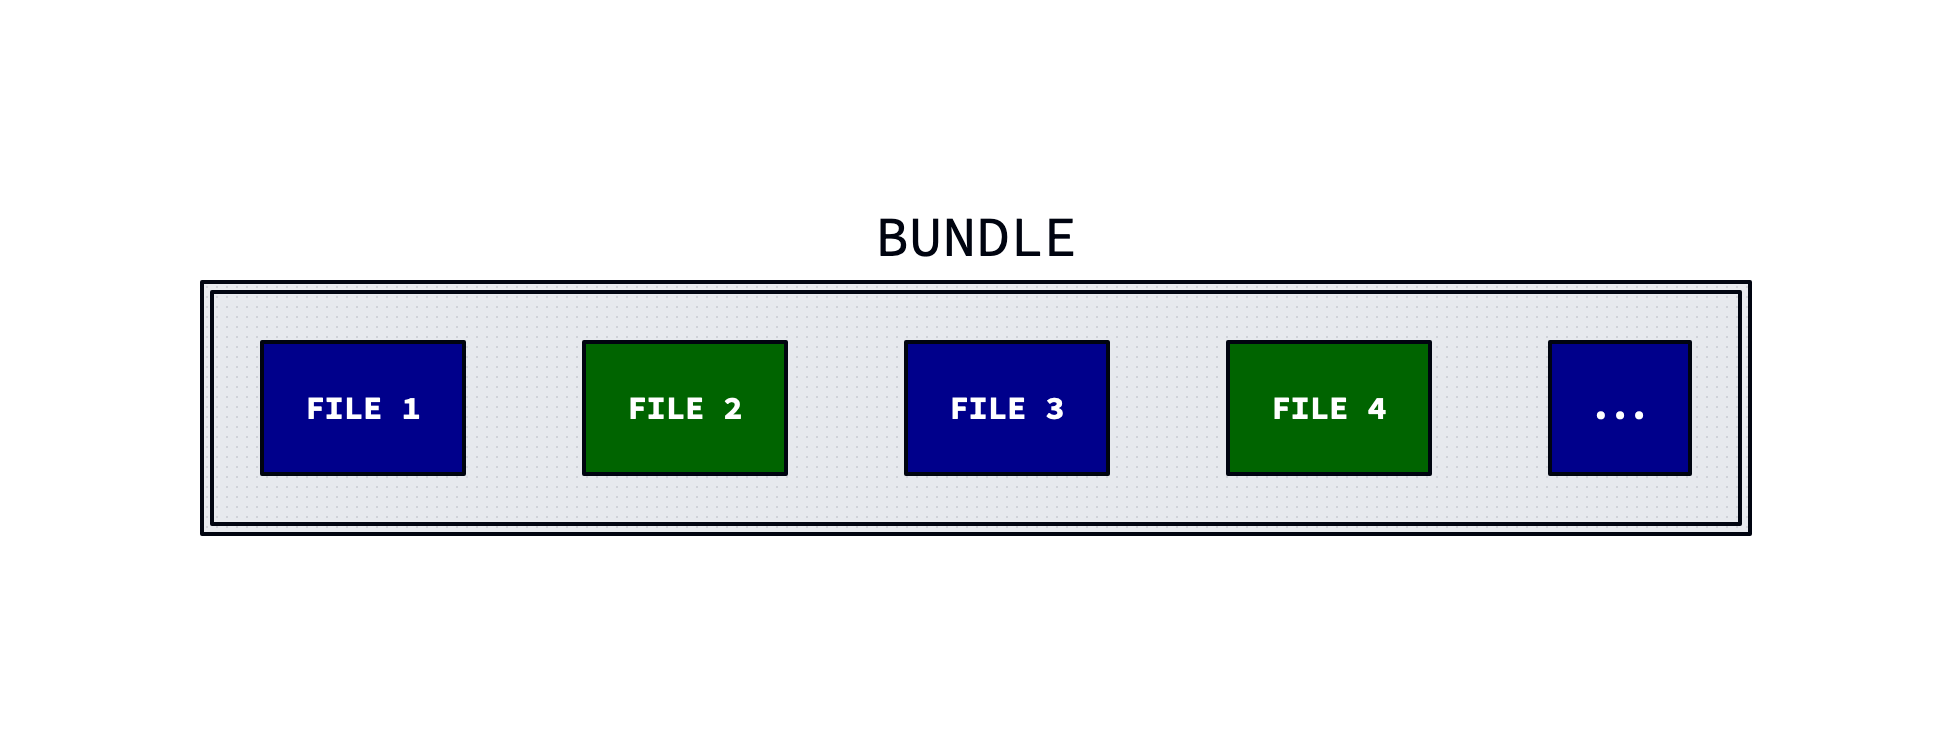
\includegraphics[width=\linewidth,height=100px]{svg/bundle.png}

    Bundling is especially efficient for object stores (e.g. S3) because the overhead for creating a new file is fairly large. Some object stores have minimum costs for storage, depending on the tier, and bundling helps ensure that files in the repository are greater than the minimum size. For example, on S3 Reduced Redundancy Storage, files smaller than 128KiB will be charged as a 128KiB file.
    \\\vspace{1em}
    The expire command also benefits because there are fewer files to remove (this is true no matter what storage is used for the repository).
\end{frame}

\begin{frame}[fragile]
    \frametitle{Block Incremental}

    Block incremental \texttt{repo-block=y} backup works by splitting the file into equal size blocks which are stored only if the block has changed. All blocks are copied for a full backup. The size of the block varies between 8KiB and 88KiB depending on the size and age of the file. Larger and older files get larger block sizes. If a file is old enough then block incremental will not be performed on it.
    \\\vspace{1em}
    Blocks are stored together in super blocks sized between 256KiB and 1MiB to improve compression efficiency.
    \\\vspace{1em}
    Each file has a map that contains the checksum of each block and where it can be found. The map is used to reconstruct the file and the checksums can be used to retrieve only the blocks that are needed for restore.
\end{frame}

\begin{frame}[fragile]
    \frametitle{Block Incremental - Full Backup}

    During a full backup all blocks are copied and a map is generated.

    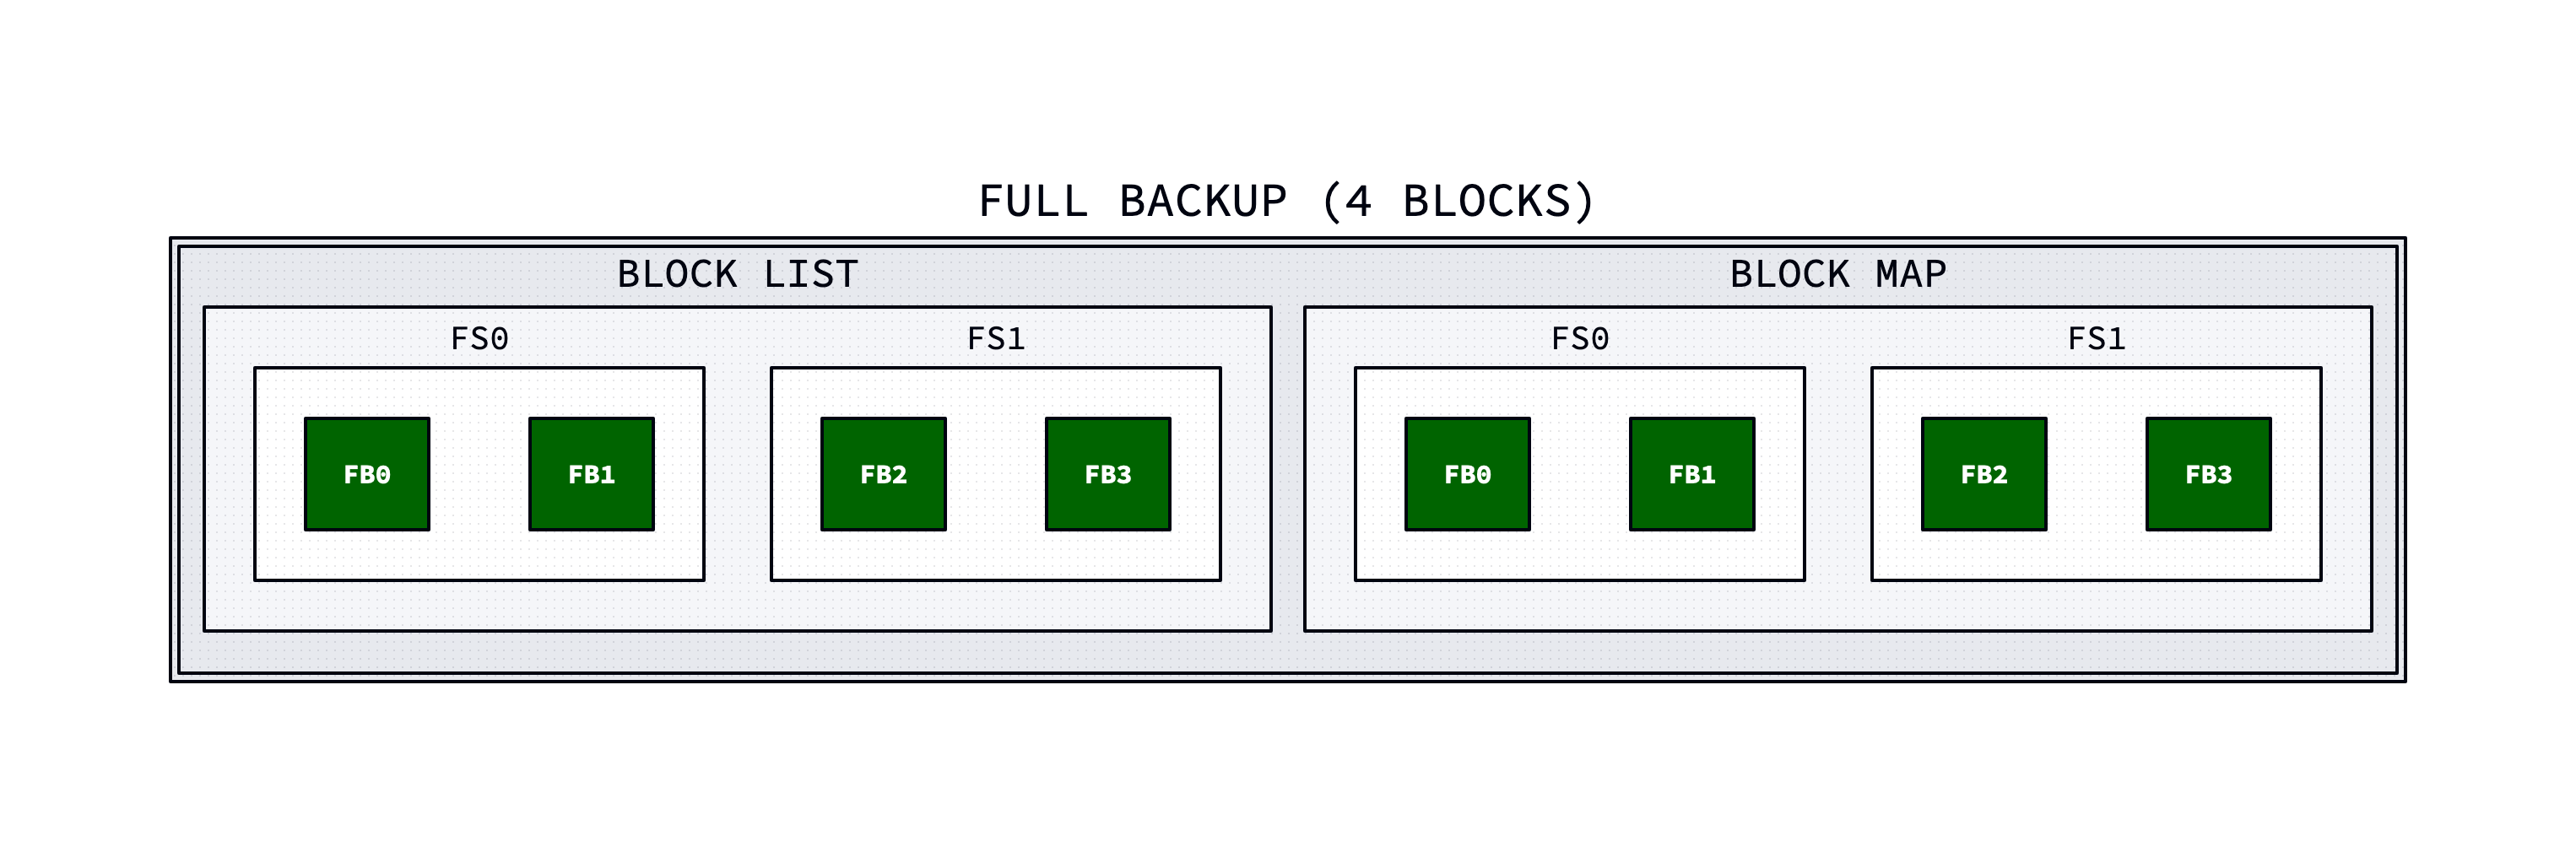
\includegraphics[width=\linewidth]{svg/block-full.png}

    This file has 4 blocks arranged into 2 superblocks of 2 blocks each. Generally there would be more blocks per superblock but this works better for demonstration purposes.
\end{frame}

\begin{frame}[fragile]
    \frametitle{Block Incremental - Differential Backup}

    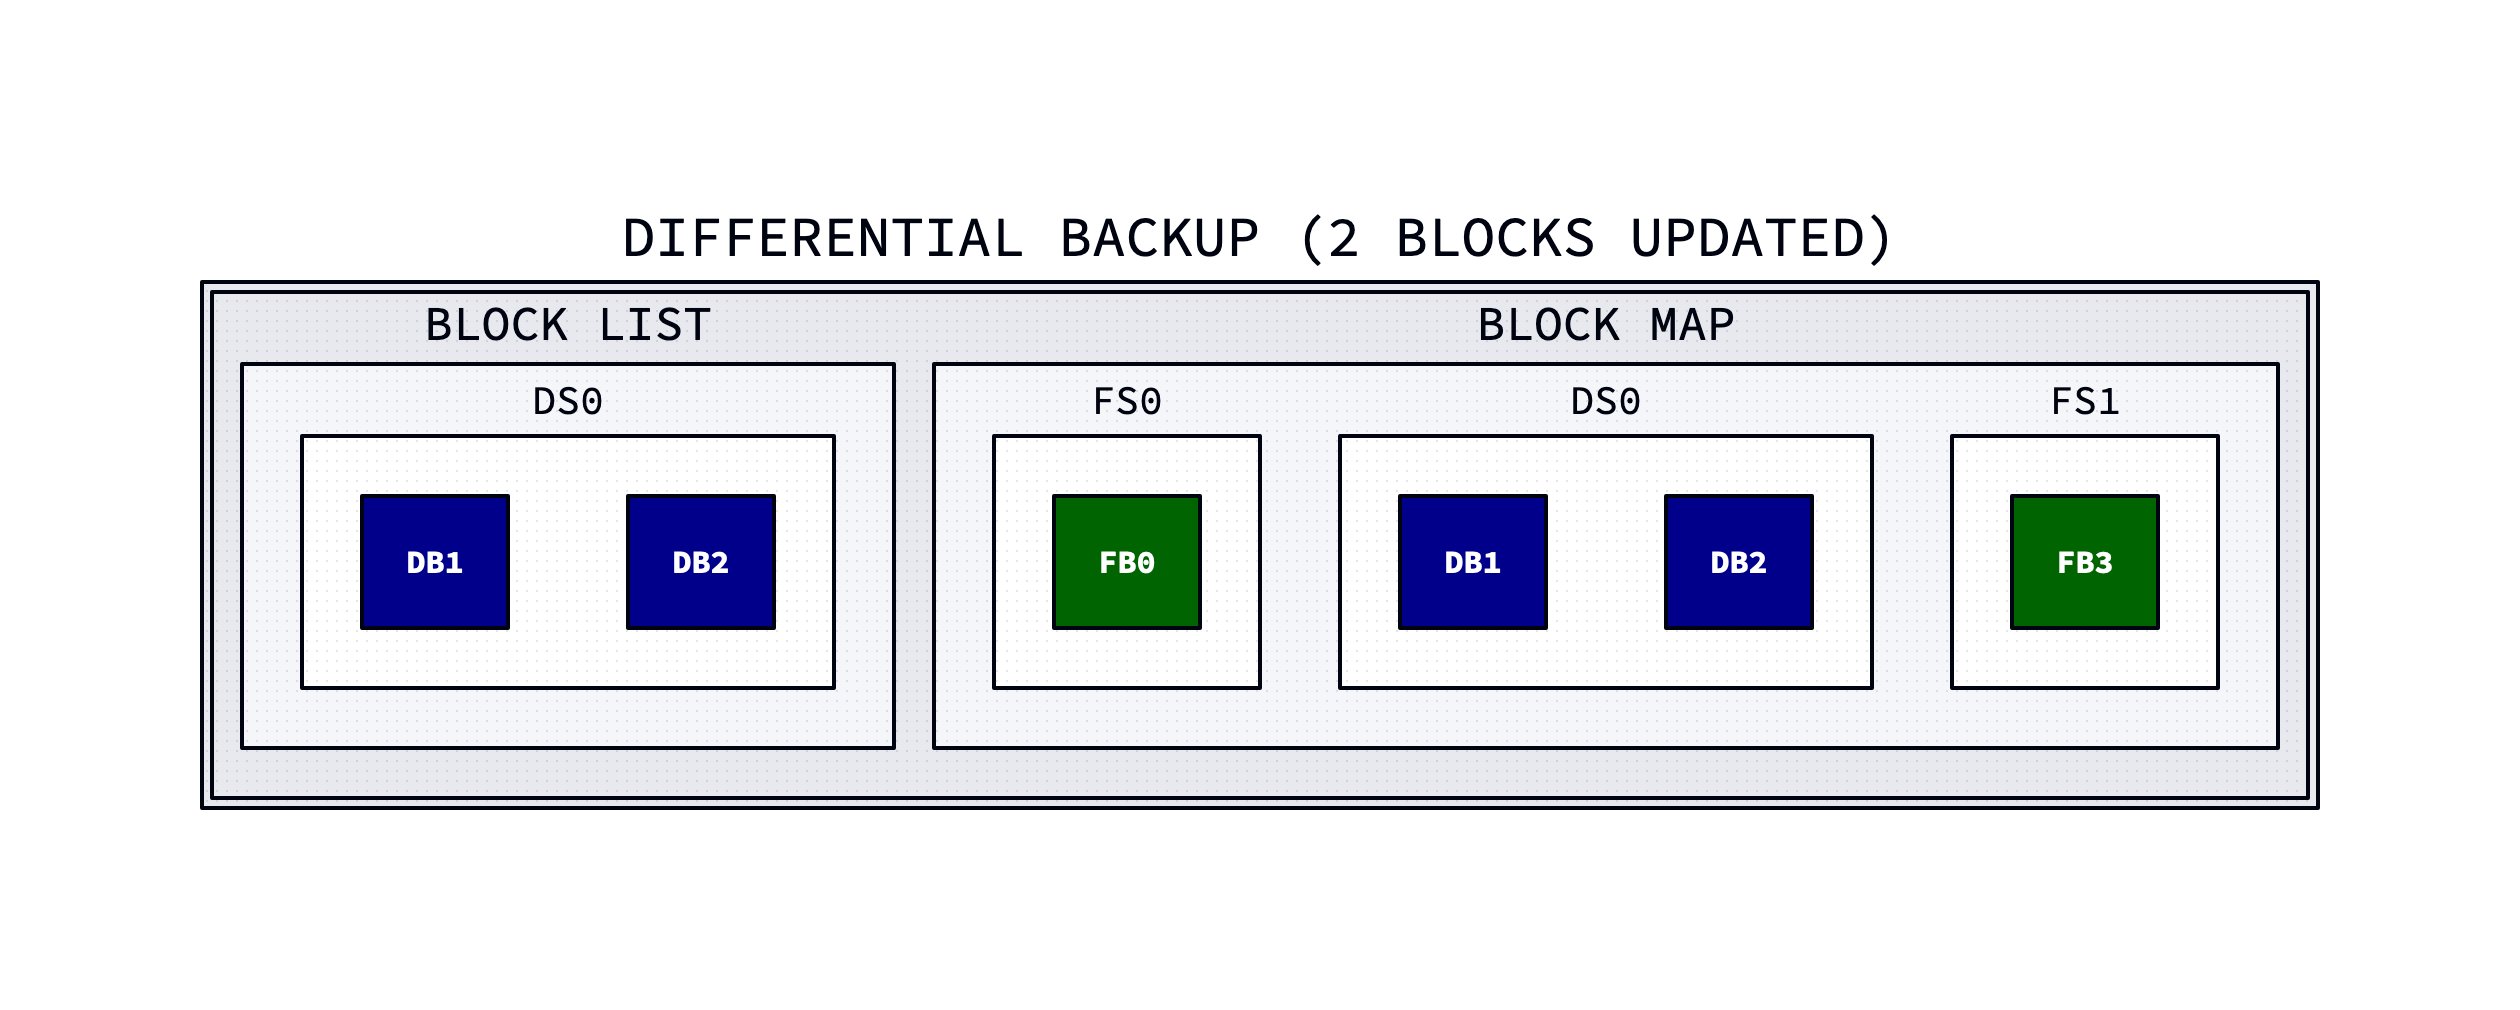
\includegraphics[width=\linewidth]{svg/block-diff.png}

    For the differential backup, the two middle blocks of the file were changed. They get stored in the block list and the map is updated with the new block references. Each time a file changes a complete copy of the map is stored with the changed blocks.
\end{frame}

\begin{frame}[fragile]
    \frametitle{Block Incremental - Incremental Backup}

    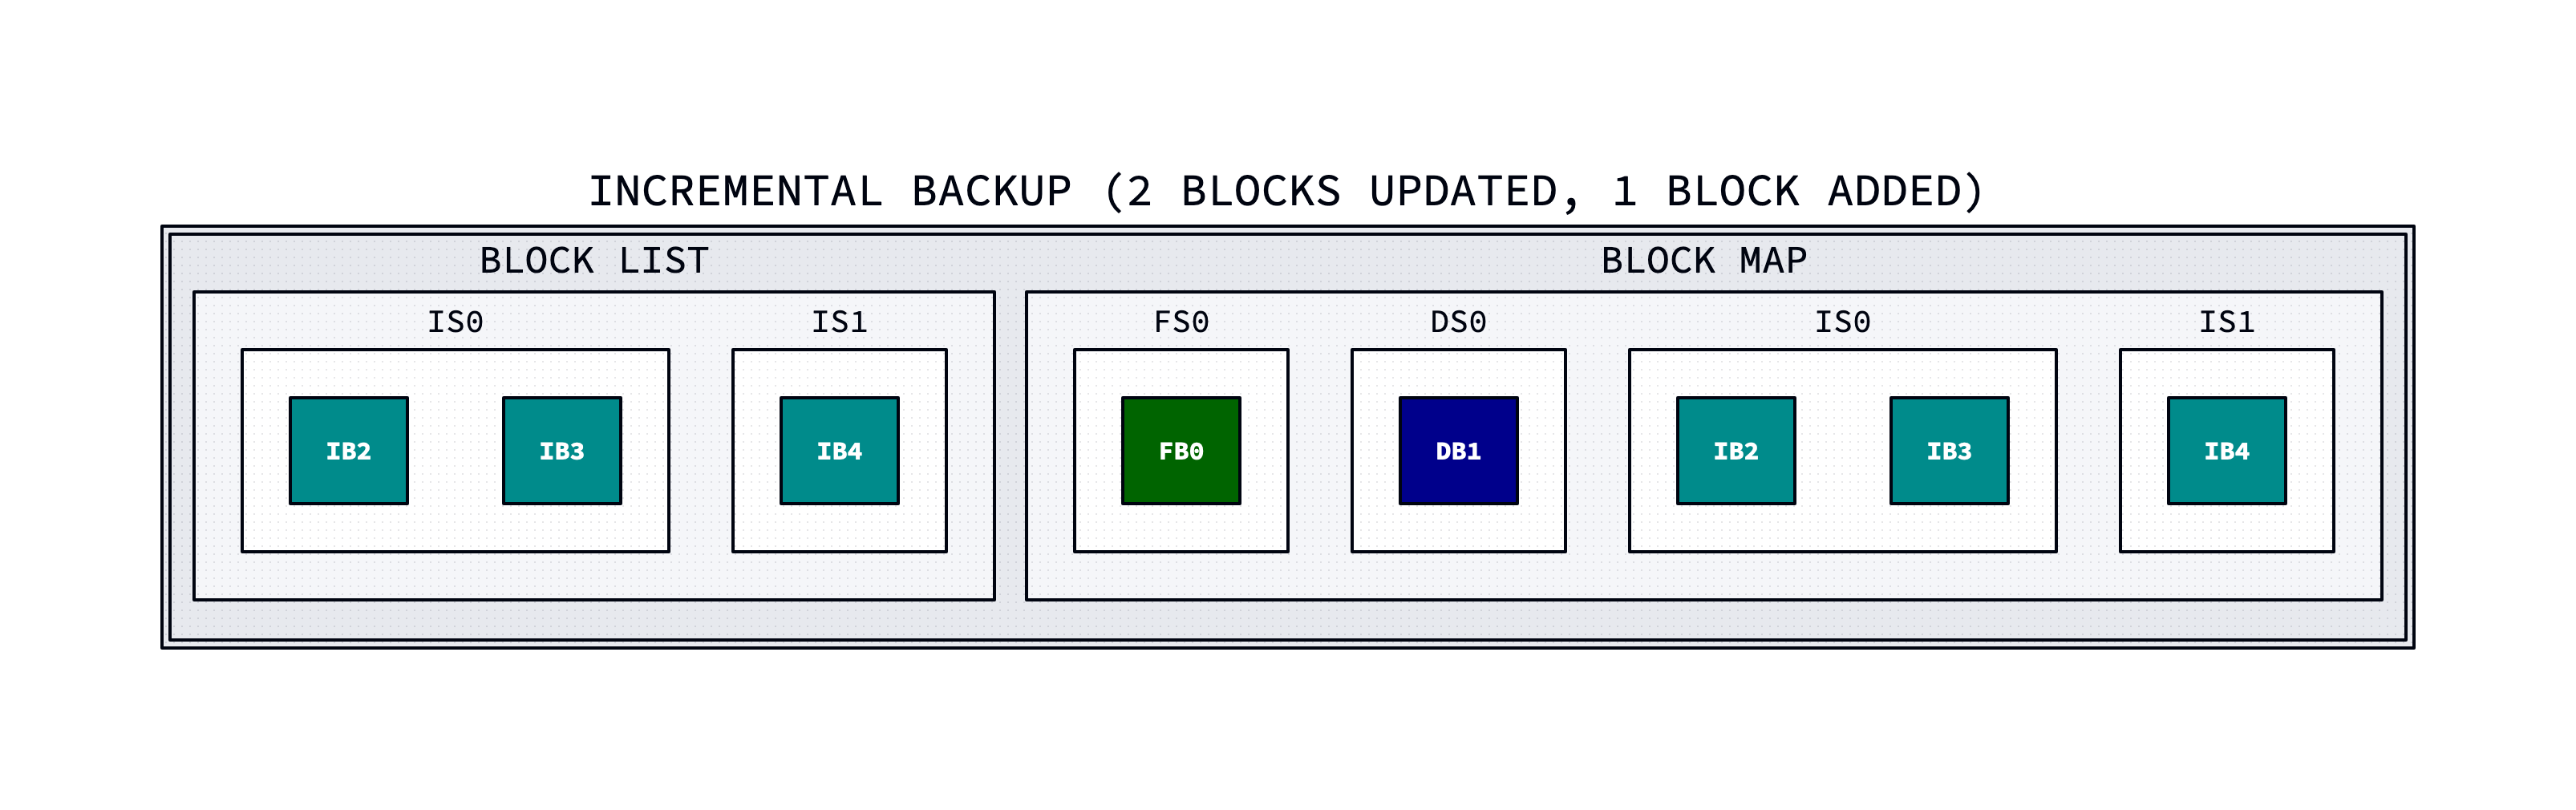
\includegraphics[width=\linewidth]{svg/block-incr.png}

    For the incremental backup, the last two blocks were changed and a block was added.
\end{frame}

\begin{frame}[fragile]
    \frametitle{Full Backup then Incremental}

    One technique to allow faster recovery of a full backup is to make an incremental backup right after a full backup, and then use that incremental for restores in preference to the full backup.
    \\\vspace{1em}
    This generally reduces the amount of WAL replay required to make the cluster consistent since the incremental backup will run for a shorter amount of time and generate less WAL.
    \\\vspace{1em}
    Note that this technique may not be as useful when performing point-in-time recovery since the WAL saved may be a small part of the total WAL that needs to be replayed to reach the recovery target.
\end{frame}

% ----------------------------------------------------------------------------------------------------------------------------------
\section{Archiving}

\begin{frame}[fragile]
    \frametitle{Asynchronous Archiving}

    Asynchronous parallel archiving (\texttt{archive-async=y}) allows compression and transfer to be offloaded to another process, which maintains continuous connections to the remote server and improves throughput significantly.
    \\\vspace{1em}
    Make sure there is enough space to hold WAL for an extended period if archiving stops.
    \\\vspace{1em}
    It is very important to monitor archiving to ensure it continues working.
\end{frame}

\begin{frame}[fragile]
    \frametitle{Archive Get Queue Max}

    When asynchronous archiving is enabled, the \texttt{archive-get} command will prefetch WAL segments and cache them locally so they can be provided to PostgreSQL very quickly when requested.
    \\\vspace{1em}
    For this to work most efficiently, pgBackRest's \texttt{spool-path} should be on the same device as PostgreSQL's \texttt{pg\_wal} directory. This allows WAL segments to be moved rather than copied, which is much faster.
    \\\vspace{1em}
    The size of \texttt{archive-get-queue-max} should be limited to 4-8GiB. Larger sizes are rarely useful unless latency to the repository (or repositories) is very high and/or \texttt{process-max=1}.
\end{frame}

\begin{frame}[fragile]
    \frametitle{Archive Push Queue Max}

    It is possible to set a maximum size (\texttt{archive-push-queue-max}) for the amount of un-archived WAL. If archiving is failing, this can prevent the disk from filling up and causing PostgreSQL to panic. This works best when WAL is on a dedicated volume -- otherwise database growth may cause PostgreSQL to run out of space instead. Set \texttt{archive-push-queue-max} to about 80\% of the volume size.
    \\\vspace{1em}
    \textbf{Use this option with caution!} While it can prevent PostgreSQL from panicking, it will also create a gap in the WAL thats will prevent point-in-time recovery from all existing backups to any point after the gap. A new backup should be made immediately after fixing the archiving issue.
\end{frame}

% ----------------------------------------------------------------------------------------------------------------------------------
\section{Restore}

\begin{frame}[fragile]
    \frametitle{Schr\"{o}dinger's Backup}

    \Large The state of any backup is unknown until a restore is attempted.
\end{frame}

\begin{frame}[fragile]
    \frametitle{Delta Restore}

    Delta restore (\texttt{delta=y}) makes restore more efficient by generating checksums of existing files on disk and comparing them to the checksums stored in the manifest. Only files with differing checksums need to be retrieved, reducing reads from the repository.
    \\\vspace{1em}
    This is ideal for rebuilding a failed node in an HA cluster before rejoining it to the cluster since many files should be unchanged since the last backup.
\end{frame}

\begin{frame}[fragile]
    \frametitle{Block Incremental Restore}

    Block incremental restore takes delta restore one step further by only retrieving parts of changed files from the repository Here is an example of reverting a single file to the full backup after the database ran for an additional day.
    \\\vspace{1em}

    \begin{quote}\begin{verbatim}
% pgbackrest manifest --pg=1 --stanza=mail \
    --filter=pg_data/base/16456/15917778.1 --set=20230917-084608F

- pg_data/base/16456/15917778.1
  size: 660.4MB, repo 469.5MB
  block: size 72KB, map size 66.0KB, checksum size 7B
  block delta:
    reference: 20230917-084608F, read: 12/13.6MB,
      superBlock: 20/20.2MB, block: 72/5MB
    \end{verbatim}\end{quote}\vspace{-1em}

    Note that reads from the repository totalled 13.6MiB to reconstruct the file, rather than 469.5MiB for the total compressed size of the file in the full backup.
\end{frame}

\begin{frame}[fragile]
    \frametitle{Block Incremental Restore (Many Incrementals)}

    Block incremental restore works best when the number of incremental backups is kept to a minimum. In this case it took more reads to restore (after 10 incremental backups) than it would have if the file had been stored without block incremental.

    \begin{verbatim}
size: 1GB, repo 71.2MB
block delta:
  reference: <...>F, rd: 1/71.1MB, sBlk: 993/1GB, blk: 6081/522.6MB
  reference: <...>F_<...>I, rd: 22/4.3MB, sBlk: 237/60.9MB, blk: 411/35.3MB
  reference: <...>F_<...>I, rd: 19/4.4MB, sBlk: 241/62.1MB, blk: 457/39.3MB
  reference: <...>F_<...>I, rd: 12/4.5MB, sBlk: 249/64MB, blk: 488/41.9MB
  <... 4 more incremental references ...>
  reference: <...>F_<...>I, rd: 2/4.8MB, sBlk: 261/67.3MB, blk: 684/58.8MB
  reference: <...>F_<...>I, rd: 1/4.7MB, sBlk: 260/67MB, blk: 731/62.8MB
  reference: <...>F_<...>I, rd: 1/4.7MB, sBlk: 258/66.5MB, blk: 774/66.5MB
  total read: 89/116.5MB, superBlock: 3488/1.6GB, block: 11916/1GB
    \end{verbatim}\vspace{-1em}

    On the other hand, the file used 121MiB in the repository (with block incremental) vs. 783MiB (without block incremental).
\end{frame}

\section{Questions?}

\begin{frame}[fragile]
    \frametitle{Questions?}

    website: \url{http://www.pgbackrest.org}\\
    \vspace{1em}
    email: \href{mailto:david@pgbackrest.org}{david@pgbackrest.org}\\
    email: \href{mailto:david@crunchydata.com}{david@crunchydata.com}\\
    \vspace{1em}
    releases: \url{https://github.com/pgbackrest/pgbackrest/releases}\\
    \vspace{1em}
    slides \& demo: \url{https://github.com/dwsteele/conference/releases}\\
\end{frame}

% End document
\end{document}
